\documentclass{article}

\usepackage[utf8]{inputenc}
\usepackage{amsmath}
\usepackage{wrapfig}
\usepackage{xfrac}
\usepackage{marginnote}
\usepackage{ulem}
\usepackage{cancel}

\usepackage{graphicx}
\usepackage{algorithm2e}
\usepackage{amssymb}
\usepackage{hyperref}
\usepackage{multirow}
\usepackage[most]{tcolorbox}
\tcbuselibrary{skins,breakable}

% \newtcolorbox{callout}[2][]{breakable,sharp corners, skin=enhancedmiddle jigsaw,parbox=false,
% boxrule=0mm,leftrule=2mm,boxsep=0mm,arc=0mm,outer arc=0mm,attach title to upper,
% after title={.\ }, coltitle=violet,colback=violet!10,colframe=violet, title={#2},
% fonttitle=\bfseries,#1}

\NewTColorBox{callout}{O{violet} m}{
  breakable,
  sharp corners,
  skin=enhancedmiddle jigsaw,
  parbox=false,
  boxrule=0mm,
  leftrule=2mm,
  boxsep=0mm,
  arc=0mm,
  outer arc=0mm,
  attach title to upper,
  after title={.\ },
  coltitle=#1,
  colback=#1!10,
  colframe=#1,
  title={#2},
  fonttitle=\bfseries,
}

\newtcolorbox{warning}[2][]{breakable,sharp corners, skin=enhancedmiddle jigsaw,parbox=false,
boxrule=0mm,leftrule=2mm,boxsep=0mm,arc=0mm,outer arc=0mm,attach title to upper,
after title={!\ }, coltitle=red,colback=red!10,colframe=red, title={#2},
fonttitle=\bfseries,#1}

\newtcolorbox{esempio}[2][]{breakable,sharp corners, skin=enhancedmiddle jigsaw,parbox=false,
boxrule=0mm,leftrule=2mm,boxsep=0mm,arc=0mm,outer arc=0mm,attach title to upper,
after title={:\ }, coltitle=blue,colback=blue!10,colframe=blue, title={#2},
fonttitle=\bfseries,#1}

\newcommand{\na}[0]{\ensuremath {\overset{N}{\rightarrow}}}
\newcommand{\rl}[3]{\inference{#1}{#2}\text{ #3}}
\newcommand{\bop}[0]{\ensuremath\oplus}
\newcommand{\appl}[2]{\ensuremath(#1)\ #2}
\newcommand{\st}[3][]{\ensuremath{\displaystyle\frac{#3\hfill}{#2\hfill} \text{#1}}}
\newcommand{\N}{\ensuremath \mathbb N}
\newcommand{\I}{\ensuremath \mathbb I}
\newcommand{\lam}[2]{\ensuremath{\lambda#1.#2}}
\newcommand{\inl}[0]{\ensuremath{\ inl\ }}
\newcommand{\inr}[0]{\ensuremath{\ inr\ }}
\newcommand{\case}[3]{\ensuremath{\text{case}#1\ \text{of}\ \left|\begin{aligned}& #2\\ & #3\end{aligned}\right.}}
\newcommand{\Da}[0]{\ensuremath{\Downarrow}}
\newcommand{\while}[2]{\ensuremath{\text{while }#1\text{ do }#2\text{ end}}}
\newcommand{\for}[3]{\ensuremath{\text{for }i=#1\text{ to }#2\text{ do }#3\text{ end}}}
\newcommand{\mE}[0]{\ensuremath{\mathbb{E}}}
\newcommand{\pair}[1]{\ensuremath{\langle#1\rangle}}
\newcommand{\V}{\ensuremath{\mathcal{V}}}
\newcommand{\cE}{\ensuremath{\mathcal{E}}}
\newcommand{\cD}{\ensuremath{\mathcal{D}}}
\newcommand{\cF}{\ensuremath{\mathcal{F}}}
\newcommand{\IF}[0]{\ensuremath {\text{ if }}}
\newcommand{\THEN}[0]{\ensuremath {\text{ then }}}
\newcommand{\ELSE}[0]{\ensuremath {\text{ else }}}
\newcommand{\AND}[0]{\ensuremath {\text{ and }}}
\newcommand{\OR}[0]{\ensuremath {\text{ or }}}
\newcommand{\unpack}[3]{\ensuremath{\text{unpack } #1 \text{ as }\langle #2 \rangle\text{ in }#3}}
\newcommand{\pack}[2]{\ensuremath{\text{pack } \pair{#1} \text{ as } #2 }}
\newcommand{\te}[1]{\text{#1}}
\newcommand{\ls}[0]{\ensuremath{\leadsto^{*}}}
\newcommand{\LET}[0]{\ensuremath{\text{ let }}}
\newcommand{\TIN}[0]{\ensuremath{\text{ in }}}
\newcommand{\NEW}[0]{\ensuremath{\text{ new }}}

\RestyleAlgo{ruled}
\SetKwComment{Comment}{//}{}
\SetKwInOut{Input}{input}
\SetKwInOut{Output}{output}
\newcommand\commentFont[1]{\ttfamily\textcolor{blue}{#1}}
\SetCommentSty{commentFont}
\normalem

\usepackage[parfill]{parskip}
\usepackage[a4paper, total={6in, 9in}]{geometry}
\usepackage{multicol}

\title{Distributed Systems - Project Report}
\author{Diego Oniarti - Alessandra Dalla Verde}
\date{Year 2024-2025}

\begin{document}

\maketitle
\tableofcontents

%\begin{multicols}{2}

\section{Design Choices}
% - nodes, clients, coordinator
% - messages (actual ones vs debug ones) + image
% - round system
% - testing (file dump, and simulation)
\subsection{System Layout}
The main classes of our system are the Nodes, the Clients, and the Coordinator.\\
The nodes and clients serve their roles as described in the project's assignment,
 while the coordinator is tasked to issue commands and enforce the project's assumptions.

To keep track of ongoing operations we implemented a ``rounds system" in which 
the coordinator issues a group of operations, waits for their conclusion, and 
repeats the process.

\subsection{Messages}
The system's components communicate through messages, divided into two main 
categories: control messages and service messages.

Control messages are exchanged instantaneously between the coordinator and the 
other actors to issue commands (requests and management operations) and to get 
their results. With this information the coordinator can guarantee that nodes 
join and leave, crash and recover one at a time, and only when there are no 
ongoing operations.

Service messages implement the actual functionalities of the system. They 
simulate the messages that would be exchanged in a real world scenario, 
hence they are only sent between nodes and clients (not the coordinator). 
To make their behaviour more realistic they are sent with a random delay, 
mimicking the propagation delay of packets.\footnote{The random delays 
\textit{could} break FIFO, but we decided to ignore this as per the project's 
given assumptions}

In \textbf{Fig.\ref{fig:messages}} we illustrate all the messages of the 
system. To reduce the number of messages we adopted the following strategies:
\begin{enumerate}
    \item \textbf{Get} and \textbf{Set}: only the nodes responsible for the 
    interested data item are contacted.
    \item \textbf{Join:} the system only asks the joining node's clockwise 
    neighbor for the data items that it is going to be responsible for, 
    avoiding a number of unnecessary message exchanges.\\
        The latest version of these data items is then obtained through the 
        Get operation. As stated above, reads already use the least 
        amount of required messages.
    \item \textbf{Leave:} the leaving node must transfer its data items to their 
    new responsible nodes. If multiple data items are sent to the same node, 
    they are bundled into the same message.
    \item \textbf{Crash:} When a node crashes it sends no messages to the 
    other nodes, only setting an internal flag. This operation is triggered 
    by a control message.
    \item \textbf{Recovery:} when a node enters recovery, it sends a data 
    request to the other nodes to get updated on the status of the system. 
    These messages are only sent to the $N-1$\footnote{N denotes the system's 
    replication factor} nodes in front and the $N-1$ nodes behind the recovering 
    one. Only these nodes may have the desired data items.
\end{enumerate}

\begin{figure}[ht!]
    \centering
    \includegraphics[width=1\linewidth]{images/messages.png}
    \caption{System messages}
    \label{fig:messages}
\end{figure}

\subsection{Round system}
There are two types of rounds: ones in which the system resolves a request (read
or write) for each client, and ones in which a node performs management 
operations (join/leave, crash/recover).

\textbf{Fig.\ref{fig:round_sys}} shows the flowchart of a system's round. The first 
diagram represents the simulation's core: the coordinator continues 
issuing operations until it reaches a stopping criterion 
and decides which type of round it must begin. The second scheme is the rounds 
final part: the coordinator waits for the operations' results and an additional 
time delay to let the system settle. Only then it will start a new round.

Fundamental variables appear in the diagrams :
\begin{itemize}
    \item \texttt{ROUNDS}: global variable indicating how many rounds the 
    coordinator must perform
    \item \texttt{ongoing\_actions}: number of pending operations for which the 
    coordinator must receive a result (success of fail); it is set based on the 
    type of round performed
    \item \texttt{nodes\_in}: list of nodes in the network
    \item \texttt{nodes\_out}: list of nodes out from the network from which the 
    coordinator chooses a joining node and in which it puts leaving nodes
    \item \texttt{crashed\_nodes}: list of crashed nodes
\end{itemize}

The coordinator updates the above lists based on the performed operations, thus 
at the begin of each round, the coordinator knows the nodes' state and it is 
able to perform actions respecting the system's requirements and assumptions.

\begin{figure}[ht!]
    \centering
    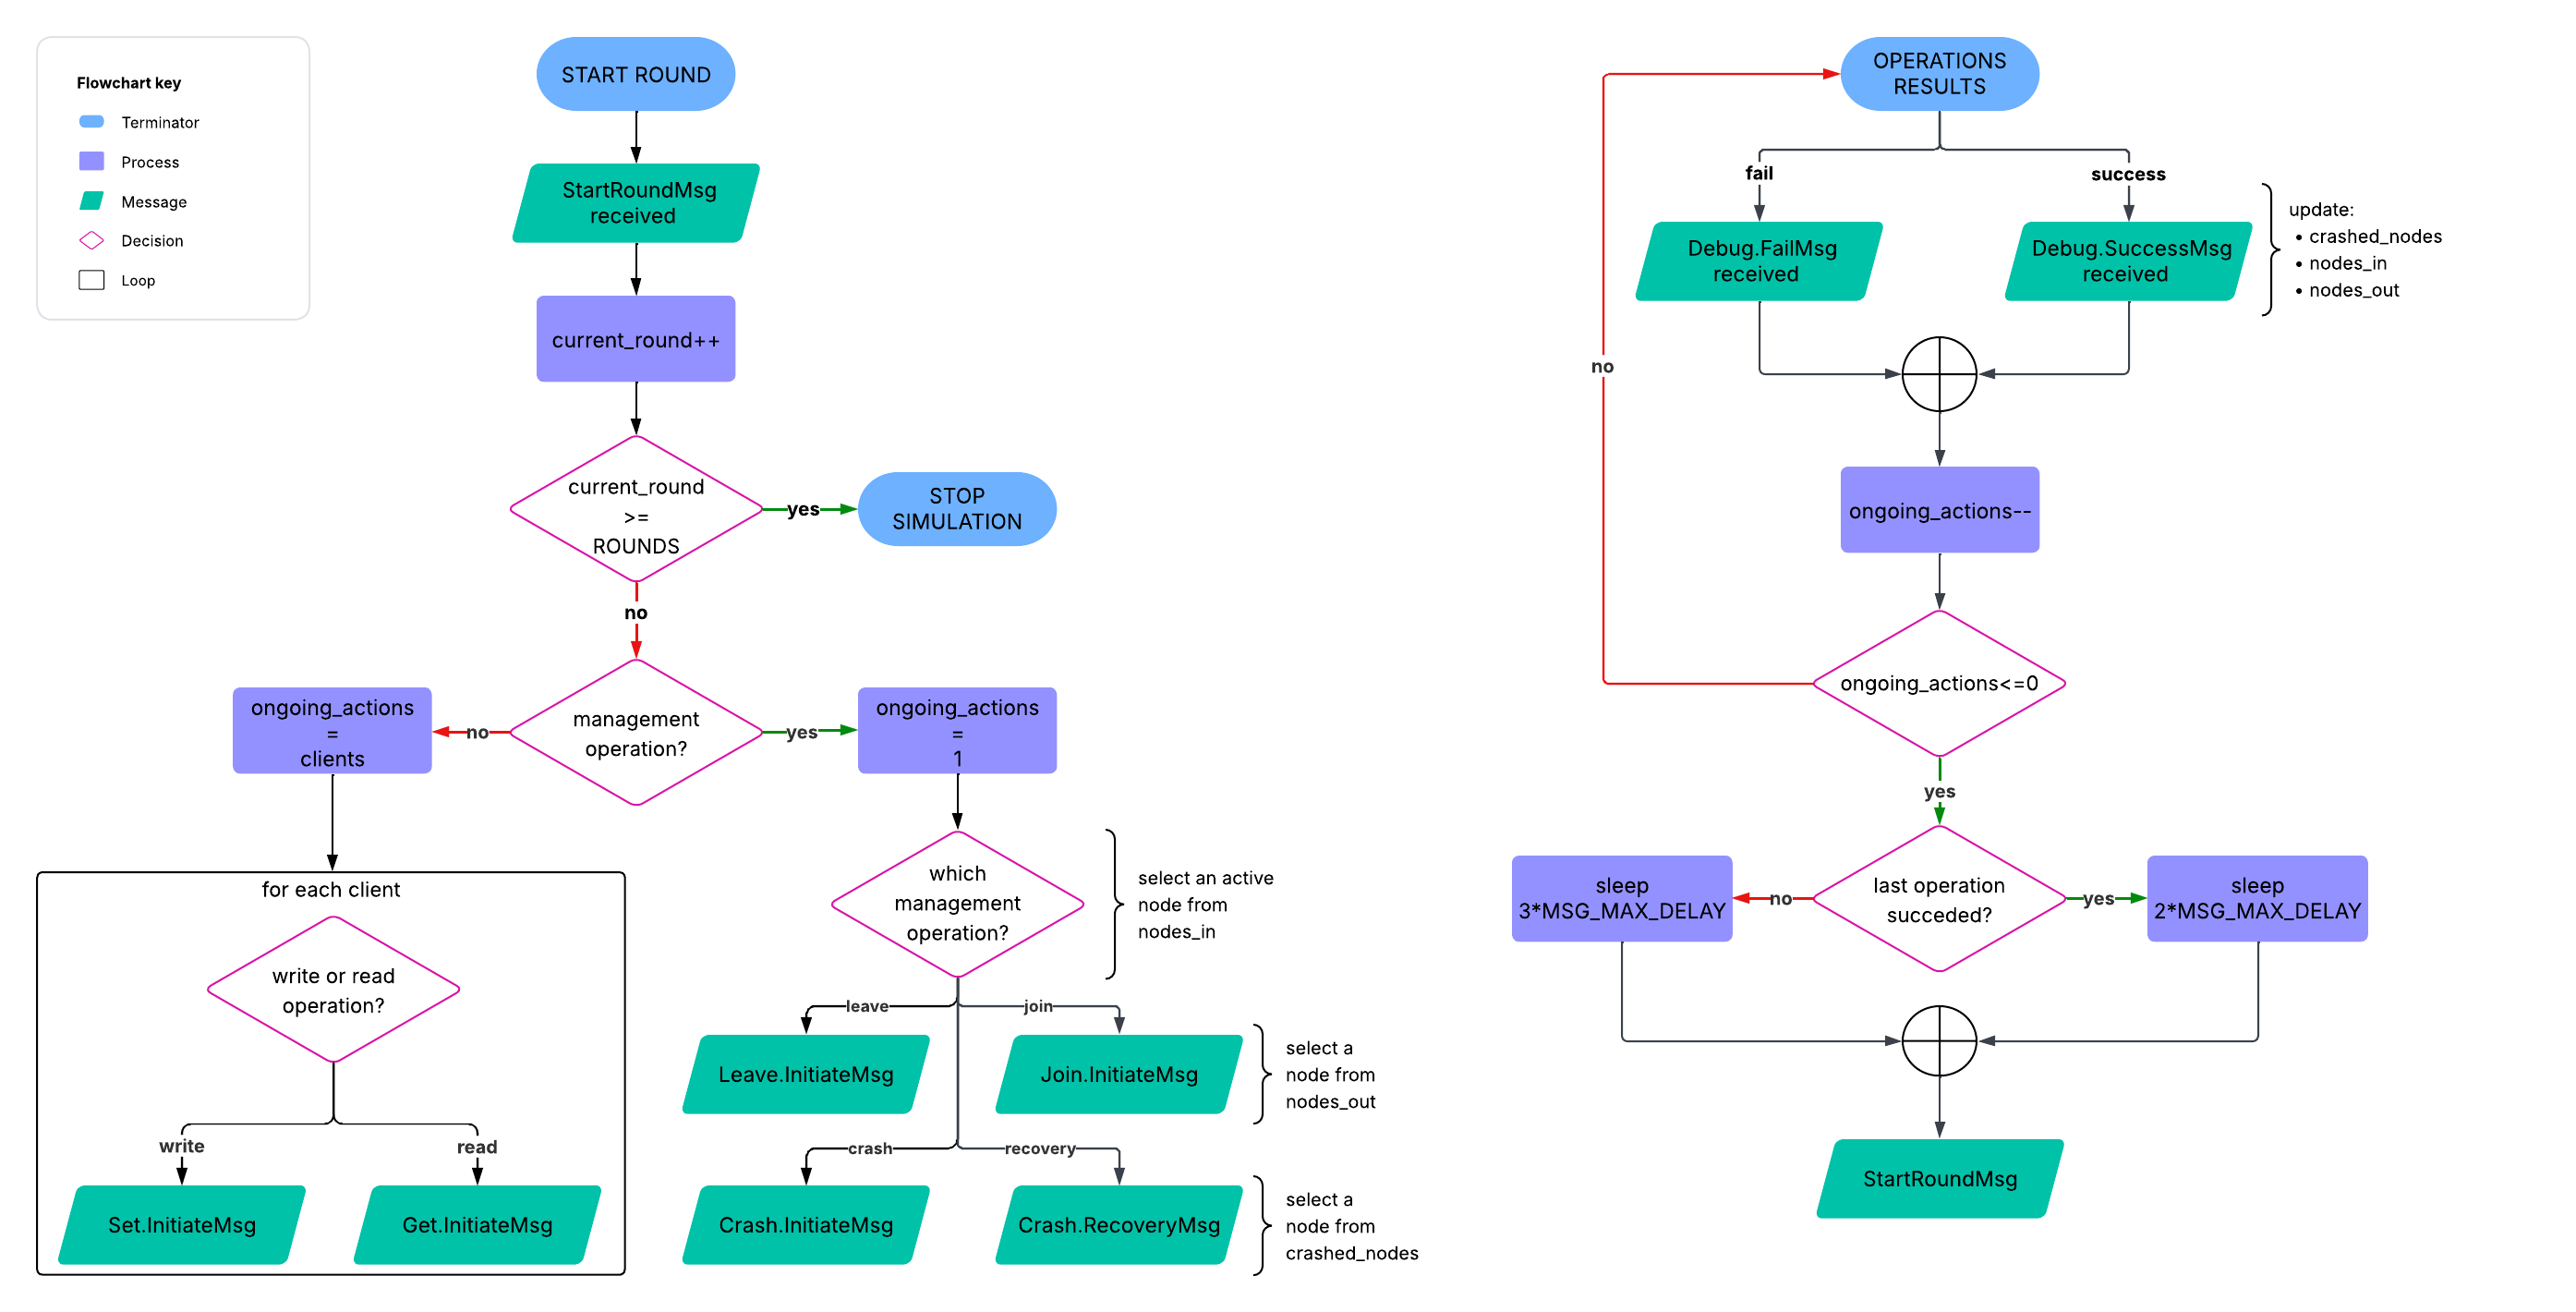
\includegraphics[width=1\linewidth]{images/round_sys.png}
    \caption{Round System}
    \label{fig:round_sys}
\end{figure}

\subsection{Crash and Recovery}
When a node crashes, it simply set an internal flag (\texttt{crashed}) and it 
stops processing messages. 

When a node recovers, it asks network topology and it requests updated versions 
of its data items. It may not receive one or more answers, in which case it
will maintain its own versions. It is not a problem, because this would only 
happen if all other nodes responsible for a data item were also crashed. If that 
were the case we can assume any other write operation would also have failed,
without modifying the data items.

\section{Assumptions and Requirements}
To ensure the system's liveliness, we made the following additional
assumptions:
\begin{itemize}
    \item clients contact an active node during set/get operations
    \item the joining node contacts an active bootstrapping peer
    \item join can fail when the node cannot read the data items it will 
    be responsible for or when the clockwise neighbor is crashed; in this last 
    case the system could stall
    \item leave can fail when the leaving node cannot share its data items
    within a given timeout
    \item a node can't leave if there are exactly $N$ nodes in the network
\end{itemize}

\subsection{Sequential Consistency}
We provided sequential consistency by managing concurrent operations and by
setting quorums appropriately.

Read/write and write/write conflicts (race conditions) are resolved by 
failing the read operation in the first case, and one of the two 
writes in the second one.

As we have seen in class, to provide sequential consistency with quorums, it is 
sufficient to set the parameters $N$, $N_{W}$, and $N_{R}$ such that:
\begin{align*}
    N_{W}&>\frac{N}{2} \\
    N_{W}+N_{R}&>N
\end{align*}

\subsection{Concurrent Transactions}
Concurrent operations could affect the system's behavior. Write/write
conflicts could cause inconsistency: responsible nodes could have the same version
but different values for for same data item. Read/write conflicts could break
sequential consistency.

We manage these conflicts in the following way:
\begin{itemize}
    \item write/write conflicts: the set transaction fails if the responsible 
    nodes for it are managing other write operations. When a node receives 
    a version request for a data item, it locks that item's key, and it no longer
    participates in any set operation on that item.
    The key is only freed when the related transaction ends (see messages of
    \texttt{set} operation in \textbf{Fig.\ref{fig:messages}}). \\
    In some corner cases it may happen that all concurrent write operations fail.
    This behaviour occurs when none of the concurrent write operations manages to
    secure enough nodes for a quorum.
    \item read/write conflicts: the get transactions fail if the responsible
    nodes are participating in a set operation on the same data item. If the
    key is locked, the node does not continue performing the read operation.
\end{itemize}

\section{Testing though Simulation}
We perform two kinds of test on the system, both performed by the AppDebug class. 
Both tests rely on a log file containing a sequence of events in their global order.

The events stored in the file are:
\begin{itemize}
    \item node storage modification: whenever data items are written or deleted 
    from a node's storage, an entry describing the change is written to the file.
    \item operations: whenever an operation succeeds or fails, it is registered 
    to the file as a single atomic entry.
\end{itemize}

\paragraph {First Test: Sequential Consistency}
A validator reads the log file and keeps track of all the successful read and write
operations, storing each one as a node in a graph. The nodes are identified
by the operation performed, the key of the item, its value, and its version.

Edges are then added between nodes to represent the happens-before relations 
between them:
\begin{enumerate}
    \item write nodes are linked to all the read nodes with the same key and 
    value, since
        a value has to be written before being read
    \item if two read events for the same key happen on the same client, an edge 
    is created
        to represent this ordering
    \item each time a client writes something, an edge between all preceding 
    read nodes (from the same client) and the
        newly formed write node is formed
\end{enumerate}
Finally, the system checks for the existence of a topological order of this 
graph, and signals an error if it can't find any.\\
If none is found, it must be because the graph contains at least one loop, which 
shouldn't happen since the edges
represent the happens-before relation which is acyclic.

If an ordering is found instead, the system enforced data-centric sequential 
consistency.

\paragraph {Second Test: Mirroring Execution}
For the second test, two replicas of the system are created, each one tracking
the individual storages of all nodes.

The first replica perfectly mirrors the execution of the real system. Data items
are added or removed from the nodes if and only if the log file states that an
alteration happened to the node's storage.

The second replica only reads the entries of the log file that report a
successful operation (be it a management one or a read/write request) and
simulates it.

The simulation keeps track of which nodes are in the system, which ones are
crashed, and updates their storages accordingly.

At the end of each round the storage of each node in the first replica is
compared with the corresponding one in the second replica. If no divergence
between the two systems is found we can confirm the actual system behaves
correctly.

\end{document}
